%  !TeX  root  =  user_guide.tex

\chapter{Working with Projections}\label{label_projections}
\index{Projections!working with}

% when the revision of a section has been finalized, 
% comment out the following line:
%\updatedisclaimer

QGIS allows users to define a global and project-wide CRS (Coordinate
Reference System) for layers without a pre-defined CRS. It also allows the
user to define custom coordinate reference systems and supports on-the-fly
(OTF) projection of vector layers. All these features allow the user to
display layers with different CRS and have them overlay properly.

\section{Overview of Projection Support}\label{label_projoverview}

QGIS has support for approximately 2,700 known CRS. Definitions for 
each of these CRS are stored in a SQLite database that is installed with
QGIS. Normally you do not need to manipulate the database directly. In fact,
doing so may cause projection support to fail. Custom CRS are stored in a
user database. See Section \ref{sec:customprojections} for
information on managing your custom coordinate reference systems.

The CRS available in QGIS are based on those defined by
EPSG\index{EPSG} and are largely abstracted from the spatial\_references 
table in PostGIS\index{PostGIS} version 1.x. The EPSG identifiers are
present in the database and can be used to specify a CRS in QGIS.

In order to use OTF projection, your data must contain information about its
coordinate reference system or you have to define a global, layer or
project-wide CRS. For PostGIS layers QGIS uses the spatial reference
identifier that was specified when the layer was created. For data supported
by OGR, QGIS relies on the presence of a format specific means of specifying
the CRS. In the case of shapefiles, this means a file containing the Well
Known Text (WKT)\index{WKT} specification of the CRS. The projection file
has the same base name as the shapefile and a prj extension. For example, a
shapefile named \filename{alaska.shp} would have a corresponding projection
file named \filename{alaska.prj}.

Whenever you select a new CRS, the used layer units will automatically be 
changed in the \tab{General} tab of the 
\dropmenuopttwo{mActionOptions}{Project Properties} dialog under the 
\mainmenuopt{Edit} (Gnome, OSX) or \mainmenuopt{Settings} (KDE, Windows) 
menu.

\section{Specifying a Projection}
\index{Projections!specifying}
\label{sec:projection-specifying}

QGIS no longer sets the map CRS to the coordinate reference system of the
first layer loaded. When you start a QGIS session with layers that do not
have a CRS, you need to control and define the CRS definition for these
layers. This can be done globally or project-wide in the \tab{CRS} tab under
\mainmenuopt{Edit} > \dropmenuopttwo{mActionOptions}{Options} (Gnome, OSX) 
or \mainmenuopt{Settings} > \dropmenuopttwo{mActionOptions}{Options} (KDE, Windows). 
See Figure~\ref{fig:crsdialog}. 

\begin{itemize}[label=--]
\item \checkbox{Prompt for CRS} 
\item \checkbox{Project wide default CRS will be used}
\item \checkbox{Global default CRS displayed below will be used}
\end{itemize}

The global default CRS \texttt{proj=longlat +ellps=WGS84 +datum=WGS84
+no\_defs} comes predefined in QGIS but can of course be changed, and the new
definition will be saved for subsequent QGIS sessions.    

\begin{figure}[ht]
   \centering
   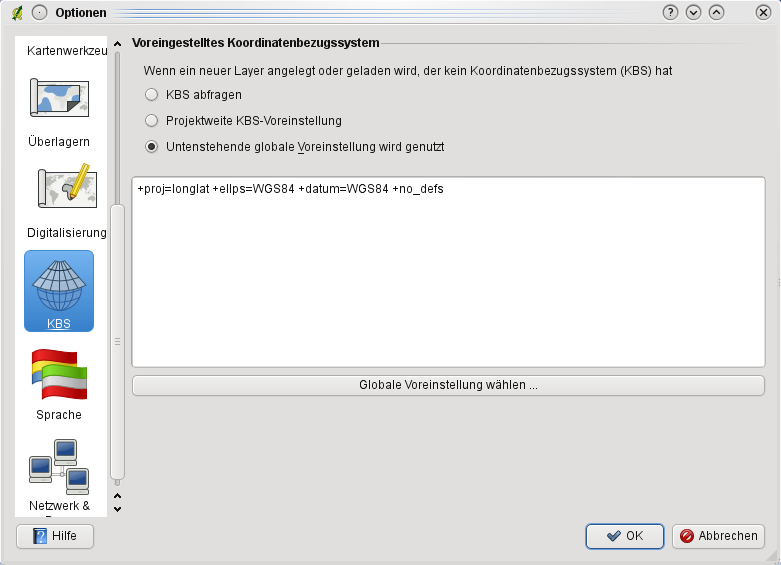
\includegraphics[clip=true, width=12cm]{crsdialog}
   \caption{CRS tab in the QGIS Options Dialog \nixcaption}\label{fig:crsdialog}
\end{figure}

If you want to define the coordinate reference system for a certain layer
without CRS information, you can also do that in the \tab{General} tab of the
raster (\ref{label_generaltab}) and vector (\ref{vectorgeneraltab}) properties 
dialog. If your layer already has a CRS defined, it
will be displayed as shown in Figure~\ref{fig:vector_symbology}.

\section{Define On The Fly (OTF) Projection}\label{label_projstart}

QGIS does not have OTF projection enabled by default, and this function is
currently only supported for vector layers. To use OTF projection, you must
open the \dropmenuopttwo{mActionOptions}{Project Properties} dialog, select a
CRS and activate the \checkbox{Enable on the fly projection} checkbox.
There are two ways to open the dialog:

\begin{enumerate}
\item Select \dropmenuopttwo{mActionOptions}{Project Properties} from the
\mainmenuopt{Edit} (Gnome, OSX) or \mainmenuopt{Settings} (KDE, Windows) menu.
\item Click on the \toolbtntwo{mIconProjectionDisabled}{projector} icon in the
lower right-hand corner of the statusbar.
\end{enumerate}

If you have already loaded a layer, and want to enable OTF projection, the
best practice is to open the \tab{Coordinate Reference System} tab of the
\dialog{Project Properties} dialog, select the CRS of the currently loaded
layer, and activate the \checkbox{Enable on the fly projection} checkbox. The
\toolbtntwo{mIconProjectionEnabled}{projector} icon will show a green hook
and all subsequently loaded vector layers will be OTF projected to the
defined CRS.
 
The \tab{Coordinate Reference System} tab of the \dialog{Project Properties}
dialog contains four important components as shown in Figure
\ref{fig:projections} and described below.

\begin{figure}[ht]
   \centering
   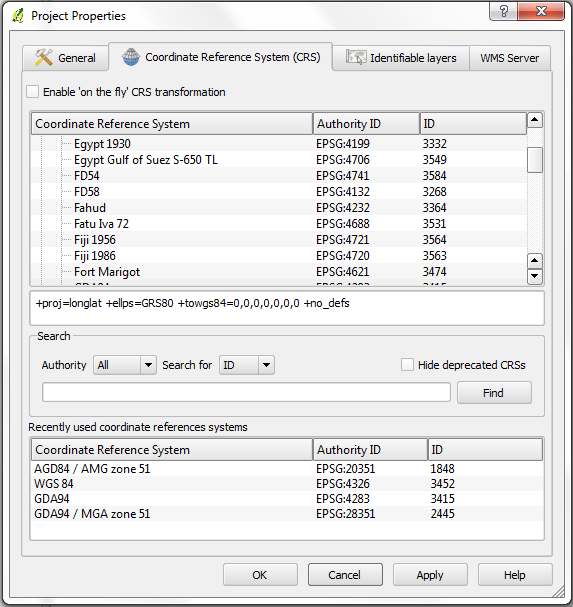
\includegraphics[clip=true, width=10cm]{projectionDialog}   
   \caption{Projection Dialog \nixcaption}\label{fig:projections}
\end{figure}

\begin{enumerate}
\item \textbf{Enable on the fly projection}\index{Projections!enabling} -
this checkbox is used to enable or disable OTF projection. When off, each
layer is drawn using the coordinates as read from the data source. When on,
the coordinates in each layer are projected to the coordinate reference
system defined for the map canvas.
\item \textbf{Coordinate Reference System} - this is a list of all CRS
supported by QGIS, including Geographic, Projected and Custom coordinate
reference systems. To use a CRS, select it from the list by expanding
the appropriate node and selecting the CRS. The active CRS is preselected.
\item \textbf{Proj4 text} - this is the CRS string used by the Proj4
projection engine. This text is read-only and provided for informational
purposes.
\item \textbf{Search} - if you know the EPSG code, the identifier or the name 
for a Coordinate Reference System, you can use the search feature to find it.
Enter the identifier and click on \button{Find}. Use the \checkbox{Hide 
deprecated CRSs} checkbox to show only the currently valid projections. 
\item \textbf{Recently used CRS} - if you have certain CRS that you frequently 
use in your everyday GIS work, these will be displayed as 'quick access' buttons 
at the bottom of the Projection Dialog. Click on one of these buttons to select 
the associated CRS.
\end{enumerate}

\begin{Tip}
\caption{\textsc{Project Properties Dialog}}
If you open the \dialog{Project Properties} dialog from the
\mainmenuopt{Edit} (Gnome, OSX) or \mainmenuopt{Settings} 
(KDE, Windows) menu, you must click on the \tab{Coordinate Reference
System} tab to view the CRS settings. Opening the dialog from the
\toolbtntwo{mIconProjectionEnabled}{projector} icon will automatically bring
the \tab{Coordinate Reference System} tab to the front.
\end{Tip}

\section{Custom Coordinate Reference System}\label{sec:customprojections}
\index{Projections!custom}

If QGIS does not provide the coordinate reference system you need, you
can define a custom CRS. To define a CRS, select
\dropmenuopttwo{mIconNew}{Custom CRS} from the \mainmenuopt{Edit} 
(Gnome, OSX) or \mainmenuopt{Settings} (KDE, Windows) menu.
Custom CRS are stored in your QGIS user database. In addition to your custom
CRS, this database also contains your spatial bookmarks and other custom data. 

\begin{figure}[ht]
   \centering
   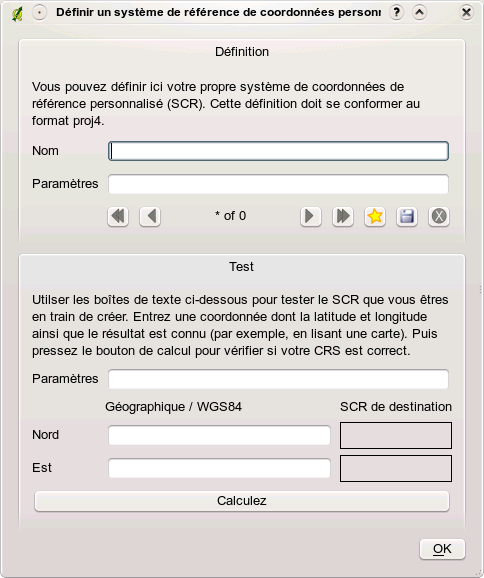
\includegraphics[clip=true, width=8cm]{customProjectionDialog}
   \caption{Custom CRS Dialog \nixcaption}\label{fig:customprojections}
\end{figure}

Defining a custom CRS in QGIS requires a good understanding of the Proj.4
projection library. To begin, refer to the Cartographic Projection Procedures
for the UNIX Environment - A User's Manual by Gerald I. Evenden, U.S.
Geological Survey Open-File Report 90-284, 1990 (available at \url{ftp://ftp.remotesensing.org/proj/OF90-284.pdf}).
This manual describes the use of the \usertext{proj.4} and related command line
utilities. The cartographic parameters used with \usertext{proj.4} are
described in the user manual, and are the same as those used by QGIS. 

The \dialog{Custom Coordinate Reference System Definition} dialog requires
only two parameters to define a user CRS: 
\begin{enumerate}
\item a descriptive name and
\item the cartographic parameters in PROJ.4 format.
\end{enumerate}
To create a new CRS, click the \toolbtntwo{mIconNew}{New} button and enter a
descriptive name and the CRS parameters. After that you can save your CRS by
clicking the button \toolbtntwo{mActionFileSave}{Save}.

Note that the \guilabel{Parameters} must begin with a \usertext{+proj=}-block,
to represent the new coordinate reference system.

You can test your CRS parameters to see if they give sane results by
clicking on the \button{Calculate} button inside the \guiheading{Test} block 
and pasting your CRS parameters into
the \guilabel{Parameters} field. Then enter known WGS 84 latitude and longitude
values in \guilabel{North} and \guilabel{East} fields respectively. 
Click on \button{Calculate} and compare the results with the known values in
your coordinate reference system.

\FloatBarrier
